\PassOptionsToPackage{unicode=true}{hyperref} % options for packages loaded elsewhere
\PassOptionsToPackage{hyphens}{url}
%
\documentclass[]{article}
\XeTeXlinebreaklocale "zh"
\XeTeXlinebreakskip = 0pt plus 1pt minus 0.1pt
\usepackage[top=1in,bottom=1in,left=1.25in,right=1.25in]{geometry}
\usepackage{float}
\usepackage{fontspec}
\newfontfamily\zhfont[BoldFont=Adobe Heiti Std]{Adobe Song Std}
\newfontfamily\zhpunctfont{Adobe Song Std}
\setmainfont{Times New Roman}
\usepackage{indentfirst}
\usepackage{zhspacing}
\zhspacing
\usepackage{lmodern}
\usepackage{amssymb,amsmath}
\usepackage{ifxetex,ifluatex}
\usepackage{fixltx2e} % provides \textsubscript
\ifnum 0\ifxetex 1\fi\ifluatex 1\fi=0 % if pdftex
  \usepackage[T1]{fontenc}
  \usepackage[utf8]{inputenc}
  \usepackage{textcomp} % provides euro and other symbols
\else % if luatex or xelatex
  \usepackage{unicode-math}
  \defaultfontfeatures{Ligatures=TeX,Scale=MatchLowercase}
\fi
% use upquote if available, for straight quotes in verbatim environments
\IfFileExists{upquote.sty}{\usepackage{upquote}}{}
% use microtype if available
\IfFileExists{microtype.sty}{%
\usepackage[]{microtype}
\UseMicrotypeSet[protrusion]{basicmath} % disable protrusion for tt fonts
}{}
\IfFileExists{parskip.sty}{%
\usepackage{parskip}
}{% else
\setlength{\parindent}{0pt}
\setlength{\parskip}{6pt plus 2pt minus 1pt}
}
\usepackage{hyperref}
\hypersetup{
            pdfborder={0 0 0},
            breaklinks=true}
\urlstyle{same}  % don't use monospace font for urls

% Fix footnotes in tables (requires footnote package)
\IfFileExists{footnote.sty}{\usepackage{footnote}\makesavenoteenv{longtable}}{}
\usepackage{graphicx,grffile}
\makeatletter
\def\maxwidth{\ifdim\Gin@nat@width>\linewidth\linewidth\else\Gin@nat@width\fi}
\def\maxheight{\ifdim\Gin@nat@height>\textheight\textheight\else\Gin@nat@height\fi}
\makeatother
% Scale images if necessary, so that they will not overflow the page
% margins by default, and it is still possible to overwrite the defaults
% using explicit options in \includegraphics[width, height, ...]{}
\setkeys{Gin}{width=\maxwidth,height=\maxheight,keepaspectratio}
\setlength{\emergencystretch}{3em}  % prevent overfull lines
\providecommand{\tightlist}{%
  \setlength{\itemsep}{0pt}\setlength{\parskip}{0pt}}
\setcounter{secnumdepth}{5}
% Redefines (sub)paragraphs to behave more like sections
\ifx\paragraph\undefined\else
\let\oldparagraph\paragraph
\renewcommand{\paragraph}[1]{\oldparagraph{#1}\mbox{}}
\fi
\ifx\subparagraph\undefined\else
\let\oldsubparagraph\subparagraph
\renewcommand{\subparagraph}[1]{\oldsubparagraph{#1}\mbox{}}
\fi

% set default figure placement to htbp
\makeatletter
\def\fps@figure{htbp}
\makeatother


\date{}

\begin{document}

\hypertarget{ux540eux7aefux63a5ux53e3ux8bf4ux660e}{%
\section{后端接口说明}\label{ux540eux7aefux63a5ux53e3ux8bf4ux660e}}

\begin{enumerate}
\def\labelenumi{\arabic{enumi}.}
\tightlist
\item
  请求参数中,若为空串均为不指定(因此大多数字段都使用了string类型)
\item
  相应的参数具有明确类型(如果int类型的就返回int类型二不是string)
\item
  都是post请求
\end{enumerate}

{[}TOC{]}

\hypertarget{ux5176ux4ed6api}{%
\subsection{其他API}\label{ux5176ux4ed6api}}

\hypertarget{apiux6211ux662fux8c01}{%
\subsubsection{API:我是谁}\label{apiux6211ux662fux8c01}}

\hypertarget{ux65b9ux6cd5}{%
\paragraph{方法}\label{ux65b9ux6cd5}}

get方法

\hypertarget{url}{%
\paragraph{URL}\label{url}}

(yb-ok) \texttt{/api/i}

\hypertarget{ux54cdux5e94ux793aux4f8bux53caux53c2ux6570}{%
\paragraph{响应示例及参数}\label{ux54cdux5e94ux793aux4f8bux53caux53c2ux6570}}

\begin{Shaded}
\begin{Highlighting}[]
\FunctionTok{\{}
    \DataTypeTok{"user_id"} \FunctionTok{:} \DecValTok{234}\FunctionTok{,}
    \DataTypeTok{"username"}\FunctionTok{:}\StringTok{"wyf"}\FunctionTok{,}
    \DataTypeTok{"role"}\FunctionTok{:}\DecValTok{0}\FunctionTok{,}
    \DataTypeTok{"error_code"}\FunctionTok{:}\DecValTok{0}
\FunctionTok{\}}
\end{Highlighting}
\end{Shaded}

\begin{longtable}[]{@{}lll@{}}
\toprule
属性名 & 类型 & 值\tabularnewline
\midrule
\endhead
user\_id & int & 用户在数据库中的唯一id\tabularnewline
username & string & 用户名\tabularnewline
role & int & 0 : root ,3 : user\tabularnewline
error\_code & int & 0 表示无异常,1表示异常\tabularnewline
\bottomrule
\end{longtable}

\hypertarget{ux623fux95f4ux9884ux8ba2ux5b50ux7cfbux7edf}{%
\subsection{房间预订子系统}\label{ux623fux95f4ux9884ux8ba2ux5b50ux7cfbux7edf}}

\hypertarget{apiux67e5ux8be2ux53efux7528ux623fux95f4}{%
\subsubsection{API:查询可用房间}\label{apiux67e5ux8be2ux53efux7528ux623fux95f4}}

\hypertarget{url-1}{%
\paragraph{URL}\label{url-1}}

(yb-ok) \texttt{/api/query\_avail\_room}

\hypertarget{ux8bf7ux6c42ux793aux4f8bux53caux53c2ux6570}{%
\paragraph{请求示例及参数}\label{ux8bf7ux6c42ux793aux4f8bux53caux53c2ux6570}}

\begin{Shaded}
\begin{Highlighting}[]
\FunctionTok{\{}
    \DataTypeTok{"check_in"}\FunctionTok{:}\StringTok{"2018-02-12"}\FunctionTok{,}
    \ErrorTok{//...以及其他属性}
\FunctionTok{\}}
\end{Highlighting}
\end{Shaded}

发送的json请求需要含有以下属性:

\begin{longtable}[]{@{}lll@{}}
\toprule
属性名 & 类型 & 值\tabularnewline
\midrule
\endhead
check\_in & string & 入住时间(\%Y-\%M-\%D 如 2018-02-12)\tabularnewline
check\_out & string & 退房时间(\%Y-\%M-\%D 如
2018-02-15)\tabularnewline
capacity & string & 最小容纳人数\tabularnewline
wifi & string &
是否要求wifi,空表示不指定,1表示必须有wifi\tabularnewline
breakfast & string &
是否要求早餐,空表示不限定,1表示必须有早餐\tabularnewline
\bottomrule
\end{longtable}

\hypertarget{ux54cdux5e94ux793aux4f8bux53caux53c2ux6570-1}{%
\paragraph{响应示例及参数}\label{ux54cdux5e94ux793aux4f8bux53caux53c2ux6570-1}}

\begin{Shaded}
\begin{Highlighting}[]
\FunctionTok{\{}
    \DataTypeTok{"rooms"}\FunctionTok{:}\OtherTok{[}
        \FunctionTok{\{}
            \DataTypeTok{"room_id"} \FunctionTok{:} \StringTok{"XXXXXX"}\FunctionTok{,}
            \DataTypeTok{"floor"} \FunctionTok{:} \DecValTok{4}\FunctionTok{,}
            \DataTypeTok{"room_num"} \FunctionTok{:} \DecValTok{1103}\FunctionTok{,}
            \DataTypeTok{"price"} \FunctionTok{:} \DecValTok{100}\FunctionTok{,}
            \DataTypeTok{"breakfast"} \FunctionTok{:} \StringTok{"Yes"}\FunctionTok{,}
            \DataTypeTok{"wifi"} \FunctionTok{:} \StringTok{"No"}\FunctionTok{,}
            \DataTypeTok{"name"} \FunctionTok{:} \StringTok{"豪华双人房"}\FunctionTok{,}
            \DataTypeTok{"capacity"} \FunctionTok{:} \DecValTok{2}
        \FunctionTok{\}}\OtherTok{,}
        \FunctionTok{\{}
            \ErrorTok{//...(同上)}
        \FunctionTok{\}}
    \OtherTok{]}
\FunctionTok{\}}
\end{Highlighting}
\end{Shaded}

\begin{longtable}[]{@{}lll@{}}
\toprule
属性名 & 类型 & 值\tabularnewline
\midrule
\endhead
room\_id & string & 房间的唯一id\tabularnewline
floor & int & 房间所在层数(1,2,3,4\ldots{}.)\tabularnewline
room\_num & int & 房间的房号(如 101,503,1103等 )\tabularnewline
price & int & 房价(单位为元)\tabularnewline
breakfast & string & `No' 表示没有早餐,'Yes'表示有早餐\tabularnewline
wifi & string & 'No'表示没有wifi,'Yes'表示有wifi\tabularnewline
name & string & 房型的名称(豪华双人房)\tabularnewline
capacity & int & 房间所能容纳的最大人数\tabularnewline
\bottomrule
\end{longtable}

\hypertarget{apiux9884ux8ba2ux623fux95f4}{%
\subsubsection{API:预订房间}\label{apiux9884ux8ba2ux623fux95f4}}

说明:已经实现了预定房间

实现说明:直接向Order表中增加一项

测试说明:使用query\_avail\_room进行测试,先使用query\_avail\_room找到某时间段内可用的房间,然后使用该接口进行预定,然后再返回查询,发现该房间果然无法再预定

\hypertarget{url-2}{%
\paragraph{URL}\label{url-2}}

(yb-ok) \texttt{/api/order\_room}

\hypertarget{ux8bf7ux6c42ux793aux4f8bux53caux53c2ux6570-1}{%
\paragraph{请求示例及参数}\label{ux8bf7ux6c42ux793aux4f8bux53caux53c2ux6570-1}}

\begin{Shaded}
\begin{Highlighting}[]
\FunctionTok{\{}
    \DataTypeTok{"check_in"}\FunctionTok{:}\StringTok{"2018-02-12"}\FunctionTok{,}
    \ErrorTok{//...以及其他属性}
\FunctionTok{\}}
\end{Highlighting}
\end{Shaded}

发送的json请求需要含有以下属性:

\begin{longtable}[]{@{}lll@{}}
\toprule
属性名 & 类型 & 值\tabularnewline
\midrule
\endhead
room\_id & int & 房间在数据库中的唯一id\tabularnewline
user\_id & int & 用户在数据库中的唯一id\tabularnewline
check\_in & string date & 入住时间(\%Y-\%M-\%D 如
2018-02-12)\tabularnewline
check\_out & string date & 退房时间(\%Y-\%M-\%D 如
2018-02-15)\tabularnewline
\bottomrule
\end{longtable}

\hypertarget{ux54cdux5e94ux793aux4f8bux53caux53c2ux6570ux8bf4ux660e}{%
\paragraph{响应示例及参数说明}\label{ux54cdux5e94ux793aux4f8bux53caux53c2ux6570ux8bf4ux660e}}

\begin{Shaded}
\begin{Highlighting}[]
\FunctionTok{\{}
    \DataTypeTok{"error_code"}\FunctionTok{:}\DecValTok{0}\FunctionTok{,}
    \DataTypeTok{"error_msg"}\FunctionTok{:}\StringTok{"ok"}
\FunctionTok{\}}
\end{Highlighting}
\end{Shaded}

\begin{longtable}[]{@{}lll@{}}
\toprule
属性名 & 类型 & 值\tabularnewline
\midrule
\endhead
errro\_code & int & 0
为无错误,1为有错误(按需求再细分错误类型)\tabularnewline
error\_msg & string & 错误信息\tabularnewline
\bottomrule
\end{longtable}

\hypertarget{ux7528ux6237ux4e2aux4ebaux5b50ux7cfbux7edf}{%
\subsection{用户个人子系统}\label{ux7528ux6237ux4e2aux4ebaux5b50ux7cfbux7edf}}

\hypertarget{apiux4feeux6539ux67d0ux4e2aux7528ux6237ux7684ux4e2aux4ebaux4fe1ux606f}{%
\subsubsection{API:修改某个用户的个人信息}\label{apiux4feeux6539ux67d0ux4e2aux7528ux6237ux7684ux4e2aux4ebaux4fe1ux606f}}

\hypertarget{url-3}{%
\paragraph{URL}\label{url-3}}

\texttt{/api/alter\_user\_info}

\hypertarget{ux8bf7ux6c42ux793aux4f8bux53caux53c2ux6570-2}{%
\paragraph{请求示例及参数}\label{ux8bf7ux6c42ux793aux4f8bux53caux53c2ux6570-2}}

\begin{Shaded}
\begin{Highlighting}[]
\FunctionTok{\{}
    \DataTypeTok{"user_id"}\FunctionTok{:} \DecValTok{1234}\FunctionTok{,}
    \DataTypeTok{"credential"}\FunctionTok{:}\StringTok{"XXXXXXX"}\FunctionTok{,}
    \DataTypeTok{"name"}\FunctionTok{:}\StringTok{"XXX"}\FunctionTok{,}
    \ErrorTok{//} \ErrorTok{...}
\FunctionTok{\}}
\end{Highlighting}
\end{Shaded}

\begin{longtable}[]{@{}lll@{}}
\toprule
属性 & 类型 & 值\tabularnewline
\midrule
\endhead
user\_id & string & 要修改信息的用户在数据库中的唯一ID\tabularnewline
credential & string & 身份证号\tabularnewline
name & string & 用户名称\tabularnewline
gender & string &
空表示不指定,'man'是雄性,'woman'是雌性\tabularnewline
birthdate & string & 用户出生日期(如``2018-01-01'')\tabularnewline
phone & string & 手机号码\tabularnewline
balance & string & 余额(单位为元)\tabularnewline
bonus & string & 积分下限\tabularnewline
\bottomrule
\end{longtable}

\hypertarget{ux54cdux5e94ux793aux4f8bux4e0eux53c2ux6570}{%
\paragraph{响应示例与参数}\label{ux54cdux5e94ux793aux4f8bux4e0eux53c2ux6570}}

\begin{verbatim}
{
    "error_code":0,
    "error_msg":"ok"
}
\end{verbatim}

\hypertarget{apiux67e5ux8be2ux81eaux5df1ux7684ux5386ux53f2ux8ba2ux5355}{%
\subsubsection{API:查询自己的历史订单}\label{apiux67e5ux8be2ux81eaux5df1ux7684ux5386ux53f2ux8ba2ux5355}}

\hypertarget{url-4}{%
\paragraph{URL}\label{url-4}}

\texttt{/api/query\_order\_by\_user}

\hypertarget{ux8bf7ux6c42ux793aux4f8bux53caux53c2ux6570-3}{%
\paragraph{请求示例及参数}\label{ux8bf7ux6c42ux793aux4f8bux53caux53c2ux6570-3}}

\begin{Shaded}
\begin{Highlighting}[]
\FunctionTok{\{}
    \DataTypeTok{"user_id"}\FunctionTok{:} \DecValTok{2342}\FunctionTok{,}
    \DataTypeTok{"check_in"}\FunctionTok{:} \StringTok{"2018-08-08"}\FunctionTok{,}
    \DataTypeTok{"check_out"}\FunctionTok{:} \StringTok{"2018-08-09"}
\FunctionTok{\}}
\end{Highlighting}
\end{Shaded}

\begin{longtable}[]{@{}lll@{}}
\toprule
属性 & 类型 & 值\tabularnewline
\midrule
\endhead
user\_id & int & user在数据库中的唯一id\tabularnewline
check\_in & string(date) & 要查询的订单的时间起点\tabularnewline
check\_out & string(date) & 要查询的订单的时间终点\tabularnewline
\bottomrule
\end{longtable}

\hypertarget{ux54cdux5e94ux793aux4f8bux4e0eux53c2ux6570-1}{%
\paragraph{响应示例与参数}\label{ux54cdux5e94ux793aux4f8bux4e0eux53c2ux6570-1}}

\begin{Shaded}
\begin{Highlighting}[]
\FunctionTok{\{}
    \DataTypeTok{"orders"}\FunctionTok{:} \OtherTok{[}
        \FunctionTok{\{}
            \DataTypeTok{"id"}\FunctionTok{:} \DecValTok{1234}\FunctionTok{,}
            \DataTypeTok{"status"}\FunctionTok{:}  \DecValTok{0}\FunctionTok{,}
            \DataTypeTok{"check_in"}\FunctionTok{:} \StringTok{"2018-08-08"}\FunctionTok{,}
            \DataTypeTok{"check_out"}\FunctionTok{:} \StringTok{"2018-08-09"}\FunctionTok{,}
            \DataTypeTok{"room_id"}\FunctionTok{:} \DecValTok{1}\FunctionTok{,}
            \DataTypeTok{"user_id"}\FunctionTok{:} \DecValTok{1}\FunctionTok{,}
        \FunctionTok{\}}\OtherTok{,}
        \FunctionTok{\{}
            \ErrorTok{//...}
        \FunctionTok{\}}
    \OtherTok{]}
\FunctionTok{\}}
\end{Highlighting}
\end{Shaded}

\begin{longtable}[]{@{}lll@{}}
\toprule
属性 & 类型 & 值\tabularnewline
\midrule
\endhead
id & int & 订单在数据库中的唯一ID\tabularnewline
status & int & 订单状态:1:已完成,0:已取消\tabularnewline
check\_in & string date & 预订的入住时间\tabularnewline
check\_out & string date & 预订的最后一天\tabularnewline
room\_id & int & 预定的房间在数据库中的唯一ID\tabularnewline
user\_id & int & 下单的用户在数据库中的唯一ID\tabularnewline
op & Array & 见下表\tabularnewline
\bottomrule
\end{longtable}

\hypertarget{apiux67e5ux8be2ux8ba2ux5355ux5173ux8054ux7684ux8be6ux60c5}{%
\subsubsection{API:查询订单关联的详情}\label{apiux67e5ux8be2ux8ba2ux5355ux5173ux8054ux7684ux8be6ux60c5}}

\hypertarget{url-5}{%
\paragraph{URL}\label{url-5}}

\texttt{/api/query\_order\_details}

\hypertarget{ux8bf7ux6c42ux793aux4f8bux53caux53c2ux6570-4}{%
\paragraph{请求示例及参数}\label{ux8bf7ux6c42ux793aux4f8bux53caux53c2ux6570-4}}

\begin{Shaded}
\begin{Highlighting}[]
\FunctionTok{\{}
    \DataTypeTok{"order_id"}\FunctionTok{:} \DecValTok{2342}
\FunctionTok{\}}
\end{Highlighting}
\end{Shaded}

\begin{longtable}[]{@{}lll@{}}
\toprule
属性 & 类型 & 值\tabularnewline
\midrule
\endhead
order\_id & int & 订单在数据库中的唯一id\tabularnewline
\bottomrule
\end{longtable}

\hypertarget{ux54cdux5e94ux793aux4f8bux4e0eux53c2ux6570-2}{%
\paragraph{响应示例与参数}\label{ux54cdux5e94ux793aux4f8bux4e0eux53c2ux6570-2}}

\begin{Shaded}
\begin{Highlighting}[]
\FunctionTok{\{}
    \DataTypeTok{"op"}\FunctionTok{:} \OtherTok{[}
    \FunctionTok{\{}
        \DataTypeTok{"id"}\FunctionTok{:} \DecValTok{2345}\FunctionTok{,}
        \DataTypeTok{"time"}\FunctionTok{:} \StringTok{"2018-08-08T15:53:00"}\FunctionTok{,}
        \DataTypeTok{"detail"}\FunctionTok{:} \DecValTok{0}\FunctionTok{,}
    \FunctionTok{\}}\OtherTok{,}
    \FunctionTok{\{}
        \ErrorTok{//...}
    \FunctionTok{\}}
\OtherTok{]}
\FunctionTok{\}}
\end{Highlighting}
\end{Shaded}

\begin{longtable}[]{@{}lll@{}}
\toprule
属性 & 类型 & 值\tabularnewline
\midrule
\endhead
id & int & 每个订单操作在数据库中的唯一ID\tabularnewline
time & string datetime & 执行操作的时间\tabularnewline
detail & int & 操作内容:1:完成订单,0:取消订单\tabularnewline
\bottomrule
\end{longtable}

\hypertarget{api-ux9000ux623f}{%
\subsubsection{API :退房}\label{api-ux9000ux623f}}

使用订单管理子系统的\texttt{cancel\_order}函数

\hypertarget{url-6}{%
\paragraph{URL}\label{url-6}}

\texttt{/api/query\_user\_info}

\hypertarget{ux7528ux6237ux6863ux6848ux5b50ux7cfbux7edf}{%
\subsection{用户档案子系统}\label{ux7528ux6237ux6863ux6848ux5b50ux7cfbux7edf}}

\hypertarget{api-ux67e5ux8be2ux6307ux5b9aux7528ux6237ux4fe1ux606f}{%
\subsubsection{API
:查询指定用户信息}\label{api-ux67e5ux8be2ux6307ux5b9aux7528ux6237ux4fe1ux606f}}

\hypertarget{url-7}{%
\paragraph{URL}\label{url-7}}

\texttt{/api/query\_user\_info}

\hypertarget{ux8bf7ux6c42ux793aux4f8bux53caux53c2ux6570-5}{%
\paragraph{请求示例及参数}\label{ux8bf7ux6c42ux793aux4f8bux53caux53c2ux6570-5}}

\begin{Shaded}
\begin{Highlighting}[]
\FunctionTok{\{}
    \DataTypeTok{"user_id"} \FunctionTok{:} \DecValTok{2342}
\FunctionTok{\}}
\end{Highlighting}
\end{Shaded}

\begin{longtable}[]{@{}lll@{}}
\toprule
属性 & 类型 & 值\tabularnewline
\midrule
\endhead
user\_id & int & user在数据库中的唯一id\tabularnewline
\bottomrule
\end{longtable}

\hypertarget{ux54cdux5e94ux793aux4f8bux4e0eux53c2ux6570-3}{%
\paragraph{响应示例与参数}\label{ux54cdux5e94ux793aux4f8bux4e0eux53c2ux6570-3}}

\begin{Shaded}
\begin{Highlighting}[]
\FunctionTok{\{}
    \DataTypeTok{"id"}\FunctionTok{:}\StringTok{"XXXX"}\FunctionTok{,}
    \DataTypeTok{"credential"}\FunctionTok{:}\StringTok{"XXXXX"}\FunctionTok{,}
    \DataTypeTok{"name"}\FunctionTok{:}\StringTok{"XXXX"}\FunctionTok{,}
    \DataTypeTok{"gender"}\FunctionTok{:}\StringTok{"man"}\FunctionTok{,}
    \DataTypeTok{"birthday"}\FunctionTok{:}\StringTok{"2018-01-01"}\FunctionTok{,}
    \DataTypeTok{"phone"}\FunctionTok{:}\StringTok{"13534343434"}\FunctionTok{,}
    \DataTypeTok{"balance"}\FunctionTok{:}\DecValTok{45}\FunctionTok{,}
    \DataTypeTok{"bonus"}\FunctionTok{:}\DecValTok{100}
\FunctionTok{\}}
\end{Highlighting}
\end{Shaded}

参数说明: \textbar{} 属性 \textbar{} 类型 \textbar{} 值 \textbar{}
\textbar{} ----------- \textbar{} ------ \textbar{}
-------------------------- \textbar{} \textbar{} id \textbar{} string
\textbar{} 用户id \textbar{} \textbar{} credential \textbar{} string
\textbar{} 身份证号 \textbar{} \textbar{} name \textbar{} string
\textbar{} 用户名称 \textbar{} \textbar{} gender \textbar{} string
\textbar{} 'man'是雄性,'woman'是雌性,空表示未知 \textbar{}
\textbar{}birthdate \textbar{} string \textbar{} 出生日期``2018-01-01''
\textbar{} \textbar{} phone \textbar{} string \textbar{} 手机号码
\textbar{} \textbar{} balance \textbar{} int \textbar{} 余额(单位为元)
\textbar{} \textbar{} bonus \textbar{} int \textbar{} 积分 \textbar{}

\hypertarget{api-ux67e5ux8be2ux6ee1ux8db3ux6761ux4ef6ux7684ux7528ux6237}{%
\subsubsection{API
:查询满足条件的用户}\label{api-ux67e5ux8be2ux6ee1ux8db3ux6761ux4ef6ux7684ux7528ux6237}}

\hypertarget{ux63a5ux53e3ux8bf4ux660e}{%
\paragraph{接口说明}\label{ux63a5ux53e3ux8bf4ux660e}}

输入一些条件,返回满足这些条件的用户列表

\begin{enumerate}
\def\labelenumi{\arabic{enumi}.}
\tightlist
\item
  string类型的参数,空串表示不指定
\end{enumerate}

\hypertarget{url-8}{%
\paragraph{URL}\label{url-8}}

(yb-ok) \texttt{/api/query\_user}

\hypertarget{ux8bf7ux6c42ux793aux4f8bux53caux53c2ux6570-6}{%
\paragraph{请求示例及参数}\label{ux8bf7ux6c42ux793aux4f8bux53caux53c2ux6570-6}}

\begin{Shaded}
\begin{Highlighting}[]
\FunctionTok{\{}
    \DataTypeTok{"credential"} \FunctionTok{:} \StringTok{"XXXXXXXXXXXXXXXXXX"}\FunctionTok{,}
    \ErrorTok{//} \ErrorTok{....} \ErrorTok{其他参数}
\FunctionTok{\}}
\end{Highlighting}
\end{Shaded}

\begin{longtable}[]{@{}lll@{}}
\toprule
属性 & 类型 & 值\tabularnewline
\midrule
\endhead
credential & string & 身份证号\tabularnewline
name & string & 用户名称\tabularnewline
gender & string &
空表示不指定,'man'是雄性,'woman'是雌性\tabularnewline
phone & string & 手机号码\tabularnewline
balance\_min & string & 余额下限(单位为元)\tabularnewline
balance\_max & string & 余额上限(单位为元)\tabularnewline
bonus\_min & string & 积分下限\tabularnewline
bonus\_max & string & 积分上限\tabularnewline
\bottomrule
\end{longtable}

\hypertarget{ux54cdux5e94ux793aux4f8bux4e0eux53c2ux6570-4}{%
\paragraph{响应示例与参数}\label{ux54cdux5e94ux793aux4f8bux4e0eux53c2ux6570-4}}

\begin{Shaded}
\begin{Highlighting}[]
\FunctionTok{\{}
    \DataTypeTok{"users"}\FunctionTok{:}\OtherTok{[}
        \FunctionTok{\{}
            \DataTypeTok{"id"}\FunctionTok{:}\StringTok{"XXXX"}\FunctionTok{,}
            \DataTypeTok{"credential"}\FunctionTok{:}\StringTok{"XXXXX"}\FunctionTok{,}
            \DataTypeTok{"name"}\FunctionTok{:}\StringTok{"XXXX"}\FunctionTok{,}
            \DataTypeTok{"gender"}\FunctionTok{:}\StringTok{"man"}\FunctionTok{,}
            \DataTypeTok{"birthday"}\FunctionTok{:}\StringTok{"2018-01-01"}\FunctionTok{,}
            \DataTypeTok{"phone"}\FunctionTok{:}\StringTok{"13534343434"}\FunctionTok{,}
            \DataTypeTok{"balance"}\FunctionTok{:}\DecValTok{45}\FunctionTok{,}
            \DataTypeTok{"bonus"}\FunctionTok{:}\DecValTok{100}
        \FunctionTok{\}}\OtherTok{,}
        \FunctionTok{\{}
            \ErrorTok{//.....}
        \FunctionTok{\}}
    \OtherTok{]}
\FunctionTok{\}}
\end{Highlighting}
\end{Shaded}

参数说明: \textbar{} 属性 \textbar{} 类型 \textbar{} 值 \textbar{}
\textbar{} ----------- \textbar{} ------ \textbar{}
-------------------------- \textbar{} \textbar{} id \textbar{} string
\textbar{} 用户id \textbar{} \textbar{} credential \textbar{} string
\textbar{} 身份证号 \textbar{} \textbar{} name \textbar{} string
\textbar{} 用户名称 \textbar{} \textbar{} gender \textbar{} string
\textbar{} 'man'是雄性,'woman'是雌性,空表示未知 \textbar{} \textbar{}
birthdate \textbar{} string \textbar{} 出生日期``2018-01-01'' \textbar{}
\textbar{} phone \textbar{} string \textbar{} 手机号码 \textbar{}
\textbar{} balance \textbar{} int \textbar{} 余额(单位为元) \textbar{}
\textbar{} bonus \textbar{} int \textbar{} 积分 \textbar{}

\hypertarget{apiux589eux52a0ux4feeux6539ux5220ux9664ux7528ux6237}{%
\subsubsection{API:增加、修改、删除用户}\label{apiux589eux52a0ux4feeux6539ux5220ux9664ux7528ux6237}}

\hypertarget{ux589eux52a0}{%
\paragraph{增加}\label{ux589eux52a0}}

\hypertarget{url-9}{%
\subparagraph{URL}\label{url-9}}

(yb-ok) \texttt{/api/insert\_user}

\hypertarget{ux8bf7ux6c42ux793aux4f8bux53caux53c2ux6570ux8bf4ux660e}{%
\subparagraph{请求示例及参数说明}\label{ux8bf7ux6c42ux793aux4f8bux53caux53c2ux6570ux8bf4ux660e}}

\begin{Shaded}
\begin{Highlighting}[]
\FunctionTok{\{}
    \DataTypeTok{"credential"}\FunctionTok{:}\StringTok{"XXXXXXX"}\FunctionTok{,}
    \DataTypeTok{"name"}\FunctionTok{:}\StringTok{"XXX"}\FunctionTok{,}
    \ErrorTok{//} \ErrorTok{...}
\FunctionTok{\}}
\end{Highlighting}
\end{Shaded}

\begin{longtable}[]{@{}lll@{}}
\toprule
属性 & 类型 & 值\tabularnewline
\midrule
\endhead
credential & string & 身份证号\tabularnewline
name & string & 用户名称\tabularnewline
gender & string &
空表示不指定,'man'是雄性,'woman'是雌性\tabularnewline
birthdate & string & 用户出生日期(如``2018-01-01'')\tabularnewline
phone & string & 手机号码\tabularnewline
balance & string & 余额(单位为元)\tabularnewline
bonus & string & 积分下限\tabularnewline
\bottomrule
\end{longtable}

\hypertarget{ux54cdux5e94ux793aux4f8bux53caux53c2ux6570ux8bf4ux660e-1}{%
\subparagraph{响应示例及参数说明}\label{ux54cdux5e94ux793aux4f8bux53caux53c2ux6570ux8bf4ux660e-1}}

\begin{Shaded}
\begin{Highlighting}[]
\FunctionTok{\{}
    \DataTypeTok{"error_code"}\FunctionTok{:}\DecValTok{0}\FunctionTok{,}
    \DataTypeTok{"error_msg"}\FunctionTok{:}\StringTok{""}
\FunctionTok{\}}
\end{Highlighting}
\end{Shaded}

\begin{longtable}[]{@{}lll@{}}
\toprule
属性名 & 类型 & 值\tabularnewline
\midrule
\endhead
errro\_code & int & 0
为无错误,1为有错误(按需求再细分错误类型)\tabularnewline
error\_msg & string & 错误信息\tabularnewline
\bottomrule
\end{longtable}

\hypertarget{ux4feeux6539}{%
\paragraph{修改}\label{ux4feeux6539}}

\hypertarget{url-10}{%
\subparagraph{URL}\label{url-10}}

(yb-ok) \texttt{/api/alter\_user\_info} \#\#\#\#\# 请求示例及参数说明

\begin{Shaded}
\begin{Highlighting}[]
\FunctionTok{\{}
    \DataTypeTok{"user_id"}\FunctionTok{:} \DecValTok{1234}\FunctionTok{,}
    \DataTypeTok{"credential"}\FunctionTok{:}\StringTok{"XXXXXXX"}\FunctionTok{,}
    \DataTypeTok{"name"}\FunctionTok{:}\StringTok{"XXX"}\FunctionTok{,}
    \ErrorTok{//} \ErrorTok{...}
\FunctionTok{\}}
\end{Highlighting}
\end{Shaded}

\begin{longtable}[]{@{}lll@{}}
\toprule
属性 & 类型 & 值\tabularnewline
\midrule
\endhead
user\_id & int & 用户在数据库中的唯一ID\tabularnewline
credential & string & 身份证号\tabularnewline
name & string & 用户名称\tabularnewline
gender & string & 空表示不指定,1(Male), 0\tabularnewline
birthdate & string & 用户出生日期(如``2018-01-01'')\tabularnewline
phone & string & 手机号码\tabularnewline
balance & string & 余额(单位为元)\tabularnewline
bonus & string & 积分下限\tabularnewline
\bottomrule
\end{longtable}

\hypertarget{ux54cdux5e94ux793aux4f8bux4e0eux53c2ux6570-5}{%
\subparagraph{响应示例与参数}\label{ux54cdux5e94ux793aux4f8bux4e0eux53c2ux6570-5}}

\begin{Shaded}
\begin{Highlighting}[]
\FunctionTok{\{}
    \DataTypeTok{"error_code"}\FunctionTok{:}\DecValTok{0}\FunctionTok{,}
    \DataTypeTok{"error_msg"}\FunctionTok{:}\StringTok{""}
\FunctionTok{\}}
\end{Highlighting}
\end{Shaded}

\begin{longtable}[]{@{}lll@{}}
\toprule
属性名 & 类型 & 值\tabularnewline
\midrule
\endhead
errro\_code & int & 0
为无错误,1为有错误(按需求再细分错误类型)\tabularnewline
error\_msg & string & 错误信息\tabularnewline
\bottomrule
\end{longtable}

\hypertarget{ux5220ux9664}{%
\paragraph{删除}\label{ux5220ux9664}}

\hypertarget{url-11}{%
\subparagraph{URL}\label{url-11}}

\texttt{/api/drop\_user} \#\#\#\#\# 请求示例及参数说明

\begin{Shaded}
\begin{Highlighting}[]
\FunctionTok{\{}
    \DataTypeTok{"user_id"}\FunctionTok{:} \DecValTok{1234}\FunctionTok{,}
\FunctionTok{\}}
\end{Highlighting}
\end{Shaded}

\begin{longtable}[]{@{}lll@{}}
\toprule
属性 & 类型 & 值\tabularnewline
\midrule
\endhead
user\_id & int & 用户在数据库中的唯一ID\tabularnewline
\bottomrule
\end{longtable}

\hypertarget{ux54cdux5e94ux793aux4f8bux4e0eux53c2ux6570-6}{%
\subparagraph{响应示例与参数}\label{ux54cdux5e94ux793aux4f8bux4e0eux53c2ux6570-6}}

\begin{Shaded}
\begin{Highlighting}[]
\FunctionTok{\{}
    \DataTypeTok{"error_code"}\FunctionTok{:}\DecValTok{0}\FunctionTok{,}
    \DataTypeTok{"error_msg"}\FunctionTok{:}\StringTok{""}
\FunctionTok{\}}
\end{Highlighting}
\end{Shaded}

\begin{longtable}[]{@{}lll@{}}
\toprule
属性名 & 类型 & 值\tabularnewline
\midrule
\endhead
errro\_code & int & 0
为无错误,1为有错误(按需求再细分错误类型)\tabularnewline
error\_msg & string & 错误信息\tabularnewline
\bottomrule
\end{longtable}

\hypertarget{ux623fux95f4ux4fe1ux606fux5b50ux7cfbux7edf}{%
\subsection{房间信息子系统}\label{ux623fux95f4ux4fe1ux606fux5b50ux7cfbux7edf}}

\hypertarget{apiux5f97ux5230ux6240ux6709ux623fux578b}{%
\subsubsection{API:得到所有房型}\label{apiux5f97ux5230ux6240ux6709ux623fux578b}}

方法:get 使用截图:

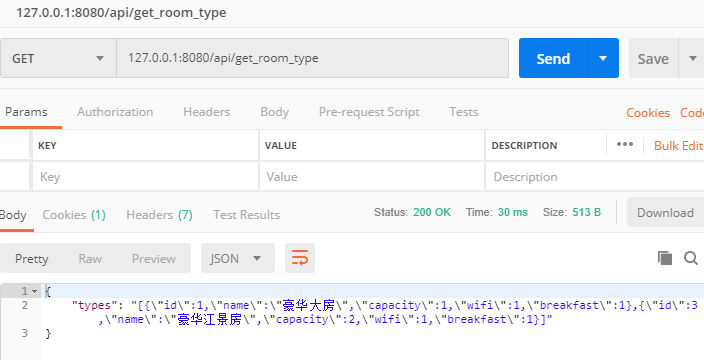
\includegraphics{figure/1544965249259.png}

\hypertarget{url-12}{%
\paragraph{URL}\label{url-12}}

(yb-ok) \texttt{/api/get\_room\_type}

\hypertarget{ux54cdux5e94ux793aux4f8bux4e0eux53c2ux6570-7}{%
\paragraph{响应示例与参数}\label{ux54cdux5e94ux793aux4f8bux4e0eux53c2ux6570-7}}

\begin{Shaded}
\begin{Highlighting}[]
\FunctionTok{\{}
    \DataTypeTok{"types"}\FunctionTok{:}\OtherTok{[}
        \StringTok{"type_id"}\ErrorTok{:}\DecValTok{1}\OtherTok{,}
        \StringTok{"name"}\ErrorTok{:}\StringTok{"豪华大房"}\OtherTok{,}
        \StringTok{"capacity"}\ErrorTok{:}\DecValTok{2}\OtherTok{,}
        \StringTok{"wifi"}\ErrorTok{:}\DecValTok{1}\OtherTok{,}
        \StringTok{"breakfast"}\ErrorTok{:}\DecValTok{0}
    \OtherTok{]}
\FunctionTok{\}}
\end{Highlighting}
\end{Shaded}

\begin{longtable}[]{@{}lll@{}}
\toprule
属性名 & 类型 & 值\tabularnewline
\midrule
\endhead
type\_id & int & 这是数据库中对房型的唯一id\tabularnewline
name & string & 这一种房间类型的名字\tabularnewline
capacity & int & 这一种房间的人数\tabularnewline
wifi & int & 0表示没有wifi,1表示有wifi\tabularnewline
breakfast & int & 0表示没有wifi,1表示有wifi\tabularnewline
\bottomrule
\end{longtable}

\hypertarget{apiux589eux52a0ux623fux95f4}{%
\subsubsection{API:增加房间}\label{apiux589eux52a0ux623fux95f4}}

\hypertarget{url-13}{%
\paragraph{URL}\label{url-13}}

(yb-ok) \texttt{/api/insert\_room}

\hypertarget{ux8bf7ux6c42ux793aux4f8bux4e0eux53c2ux6570}{%
\paragraph{请求示例与参数}\label{ux8bf7ux6c42ux793aux4f8bux4e0eux53c2ux6570}}

\begin{Shaded}
\begin{Highlighting}[]
\FunctionTok{\{}
    \DataTypeTok{"floor"}\FunctionTok{:}\DecValTok{3}\FunctionTok{,}
    \DataTypeTok{"room_num"}\FunctionTok{:}\StringTok{"304"}\FunctionTok{,}
    \DataTypeTok{"price"}\FunctionTok{:}\DecValTok{100}\FunctionTok{,}
    \DataTypeTok{"type_id"}\FunctionTok{:}\DecValTok{4}
\FunctionTok{\}}
\end{Highlighting}
\end{Shaded}

\begin{longtable}[]{@{}lll@{}}
\toprule
属性名 & 类型 & 值\tabularnewline
\midrule
\endhead
floor & int & 该房间的层数\tabularnewline
room\_num & string & 房号\tabularnewline
price & int & 房间的价格(元/每晚)\tabularnewline
type\_id & int & 房间类型的id,与RoomType表内的id对应\tabularnewline
\bottomrule
\end{longtable}

\hypertarget{ux76f8ux5e94ux793aux4f8bux4e0eux53c2ux6570}{%
\paragraph{相应示例与参数}\label{ux76f8ux5e94ux793aux4f8bux4e0eux53c2ux6570}}

\begin{Shaded}
\begin{Highlighting}[]
\FunctionTok{\{}
    \DataTypeTok{"error_code"}\FunctionTok{:}\DecValTok{0}\FunctionTok{,}
    \DataTypeTok{"error_msg"}\FunctionTok{:}\StringTok{"XXX"}
\FunctionTok{\}}
\end{Highlighting}
\end{Shaded}

\begin{longtable}[]{@{}lll@{}}
\toprule
属性名 & 类型 & 值\tabularnewline
\midrule
\endhead
error\_code & int & 0表示无异常,1表示发生错误\tabularnewline
error\_msg & string & 错误信息\tabularnewline
\bottomrule
\end{longtable}

\hypertarget{apiux51cfux5c11ux623fux95f4}{%
\subsubsection{API:减少房间}\label{apiux51cfux5c11ux623fux95f4}}

\hypertarget{url-14}{%
\paragraph{URL}\label{url-14}}

\texttt{/api/drop\_room}

\hypertarget{ux8bf7ux6c42ux793aux4f8bux4e0eux53c2ux6570-1}{%
\paragraph{请求示例与参数}\label{ux8bf7ux6c42ux793aux4f8bux4e0eux53c2ux6570-1}}

\begin{Shaded}
\begin{Highlighting}[]
\FunctionTok{\{}
    \DataTypeTok{"room_id"}\FunctionTok{:}\DecValTok{3}
\FunctionTok{\}}
\end{Highlighting}
\end{Shaded}

\begin{longtable}[]{@{}lll@{}}
\toprule
属性名 & 类型 & 值\tabularnewline
\midrule
\endhead
room\_id & int & 房间的id\tabularnewline
\bottomrule
\end{longtable}

\hypertarget{ux76f8ux5e94ux793aux4f8bux4e0eux53c2ux6570-1}{%
\paragraph{相应示例与参数}\label{ux76f8ux5e94ux793aux4f8bux4e0eux53c2ux6570-1}}

\begin{Shaded}
\begin{Highlighting}[]
\FunctionTok{\{}
    \DataTypeTok{"error_code"}\FunctionTok{:}\DecValTok{0}\FunctionTok{,}
    \DataTypeTok{"error_msg"}\FunctionTok{:}\StringTok{"XXX"}
\FunctionTok{\}}
\end{Highlighting}
\end{Shaded}

\begin{longtable}[]{@{}lll@{}}
\toprule
属性名 & 类型 & 值\tabularnewline
\midrule
\endhead
error\_code & int & 0表示无异常,1表示发生错误\tabularnewline
error\_msg & string & 错误信息\tabularnewline
\bottomrule
\end{longtable}

\hypertarget{apiux4feeux6539ux623fux95f4}{%
\subsubsection{API:修改房间}\label{apiux4feeux6539ux623fux95f4}}

\hypertarget{url-15}{%
\paragraph{URL}\label{url-15}}

\texttt{/api/alter\_room}

\hypertarget{ux8bf7ux6c42ux793aux4f8bux4e0eux53c2ux6570-2}{%
\paragraph{请求示例与参数}\label{ux8bf7ux6c42ux793aux4f8bux4e0eux53c2ux6570-2}}

\begin{Shaded}
\begin{Highlighting}[]
\FunctionTok{\{}
    \DataTypeTok{"room_id"}\FunctionTok{:}\DecValTok{3}\FunctionTok{,}
    \DataTypeTok{"floor"}\FunctionTok{:}\DecValTok{3}\FunctionTok{,}
    \DataTypeTok{"room_num"}\FunctionTok{:}\StringTok{"304"}\FunctionTok{,}
    \DataTypeTok{"price"}\FunctionTok{:}\DecValTok{100}\FunctionTok{,}
    \DataTypeTok{"type_id"}\FunctionTok{:}\DecValTok{4}
\FunctionTok{\}}
\end{Highlighting}
\end{Shaded}

\begin{longtable}[]{@{}lll@{}}
\toprule
属性名 & 类型 & 值\tabularnewline
\midrule
\endhead
room\_id & int & 房间的id\tabularnewline
floor & int & 该房间的层数\tabularnewline
room\_num & string & 房号\tabularnewline
price & int & 房间的价格(元/每晚)\tabularnewline
type\_id & int & 房间类型的id,与RoomType表内的id对应\tabularnewline
\bottomrule
\end{longtable}

\hypertarget{ux76f8ux5e94ux793aux4f8bux4e0eux53c2ux6570-2}{%
\paragraph{相应示例与参数}\label{ux76f8ux5e94ux793aux4f8bux4e0eux53c2ux6570-2}}

\begin{Shaded}
\begin{Highlighting}[]
\FunctionTok{\{}
    \DataTypeTok{"error_code"}\FunctionTok{:}\DecValTok{0}\FunctionTok{,}
    \DataTypeTok{"error_msg"}\FunctionTok{:}\StringTok{"XXX"}
\FunctionTok{\}}
\end{Highlighting}
\end{Shaded}

\begin{longtable}[]{@{}lll@{}}
\toprule
属性名 & 类型 & 值\tabularnewline
\midrule
\endhead
error\_code & int & 0表示无异常,1表示发生错误\tabularnewline
error\_msg & string & 错误信息\tabularnewline
\bottomrule
\end{longtable}

\hypertarget{apiux589eux52a0ux623fux578b}{%
\subsubsection{API:增加房型}\label{apiux589eux52a0ux623fux578b}}

\hypertarget{url-16}{%
\paragraph{URL}\label{url-16}}

(yb-ok) \texttt{/api/insert\_room\_type}

\hypertarget{ux8bf7ux6c42ux5b9eux4f8bux4e0eux53c2ux6570}{%
\paragraph{请求实例与参数}\label{ux8bf7ux6c42ux5b9eux4f8bux4e0eux53c2ux6570}}

\begin{longtable}[]{@{}lll@{}}
\toprule
属性名 & 类型 & 值\tabularnewline
\midrule
\endhead
name & string & 这一种房间类型的名字\tabularnewline
capacity & int & 这一种房间的人数\tabularnewline
wifi & int & 0表示没有wifi,1表示有wifi\tabularnewline
breakfast & int & 0表示没有wifi,1表示有wifi\tabularnewline
\bottomrule
\end{longtable}

\hypertarget{ux54cdux5e94ux793aux4f8bux4e0eux53c2ux6570-8}{%
\paragraph{响应示例与参数}\label{ux54cdux5e94ux793aux4f8bux4e0eux53c2ux6570-8}}

\begin{longtable}[]{@{}lll@{}}
\toprule
属性名 & 类型 & 值\tabularnewline
\midrule
\endhead
error\_code & int & 0为正常,1为异常\tabularnewline
error\_msg & string & 错误信息\tabularnewline
\bottomrule
\end{longtable}

\hypertarget{apiux51cfux5c11ux623fux578b}{%
\subsubsection{API:减少房型}\label{apiux51cfux5c11ux623fux578b}}

\hypertarget{url-17}{%
\paragraph{URL}\label{url-17}}

\texttt{/api/drop\_room\_type}

\hypertarget{ux8bf7ux6c42ux793aux4f8bux4e0eux53c2ux6570-3}{%
\paragraph{请求示例与参数}\label{ux8bf7ux6c42ux793aux4f8bux4e0eux53c2ux6570-3}}

\begin{longtable}[]{@{}lll@{}}
\toprule
属性 & 类型 & 值\tabularnewline
\midrule
\endhead
type\_id & int & 这是数据库中对房型的唯一id\tabularnewline
\bottomrule
\end{longtable}

\hypertarget{ux54cdux5e94ux793aux4f8bux4e0eux53c2ux6570-9}{%
\paragraph{响应示例与参数}\label{ux54cdux5e94ux793aux4f8bux4e0eux53c2ux6570-9}}

\begin{longtable}[]{@{}lll@{}}
\toprule
属性名 & 类型 & 值\tabularnewline
\midrule
\endhead
error\_code & int & 0为正常,1为异常\tabularnewline
error\_msg & string & 错误信息\tabularnewline
\bottomrule
\end{longtable}

\hypertarget{apiux4feeux6539ux623fux578b}{%
\subsubsection{API:修改房型}\label{apiux4feeux6539ux623fux578b}}

\hypertarget{url-18}{%
\paragraph{URL}\label{url-18}}

\texttt{/api/alter\_room\_type}

\hypertarget{ux8bf7ux6c42ux5b9eux4f8bux4e0eux53c2ux6570-1}{%
\paragraph{请求实例与参数}\label{ux8bf7ux6c42ux5b9eux4f8bux4e0eux53c2ux6570-1}}

\begin{Shaded}
\begin{Highlighting}[]
\FunctionTok{\{}
    \ErrorTok{'type_id'}\FunctionTok{:} \DecValTok{1}\FunctionTok{,}
    \ErrorTok{'name'}\FunctionTok{:} \ErrorTok{'豪华总统房'}\FunctionTok{,}
    \ErrorTok{//......}
\FunctionTok{\}}
\end{Highlighting}
\end{Shaded}

\begin{longtable}[]{@{}lll@{}}
\toprule
属性名 & 类型 & 值\tabularnewline
\midrule
\endhead
type\_id & int & 这是数据库中对房型的唯一id\tabularnewline
name & string & 这一种房间类型的名字\tabularnewline
capacity & int & 这一种房间的人数\tabularnewline
wifi & int & 0表示没有wifi,1表示有wifi\tabularnewline
breakfast & int & 0表示没有wifi,1表示有wifi\tabularnewline
\bottomrule
\end{longtable}

\hypertarget{ux54cdux5e94ux793aux4f8bux4e0eux53c2ux6570-10}{%
\paragraph{响应示例与参数}\label{ux54cdux5e94ux793aux4f8bux4e0eux53c2ux6570-10}}

\begin{longtable}[]{@{}lll@{}}
\toprule
属性名 & 类型 & 值\tabularnewline
\midrule
\endhead
error\_code & int & 0为正常,1为异常\tabularnewline
error\_msg & string & 错误信息\tabularnewline
\bottomrule
\end{longtable}

\hypertarget{apiux67e5ux8be2ux6ee1ux8db3ux6761ux4ef6ux7684ux623fux95f4}{%
\subsubsection{API:查询满足条件的房间}\label{apiux67e5ux8be2ux6ee1ux8db3ux6761ux4ef6ux7684ux623fux95f4}}

\hypertarget{url-19}{%
\paragraph{URL}\label{url-19}}

(yb-ok) \texttt{/api/query\_avail\_room} \#\#\#\# 请求实例与参数

\begin{Shaded}
\begin{Highlighting}[]
\FunctionTok{\{}
    \ErrorTok{'check_in'}\FunctionTok{:} \ErrorTok{'}\DecValTok{2019-01-15}\ErrorTok{'}\FunctionTok{,}
    \ErrorTok{'check_out'}\FunctionTok{:} \ErrorTok{'}\DecValTok{2019-1-17}\ErrorTok{'}\FunctionTok{,}
    \ErrorTok{'capacity'}\FunctionTok{:} \ErrorTok{''}\FunctionTok{,}
    \ErrorTok{'wifi'}\FunctionTok{:} \ErrorTok{''}\FunctionTok{,}
    \ErrorTok{'breakfast'}\FunctionTok{:} \ErrorTok{'}\DecValTok{1}\ErrorTok{'}
\FunctionTok{\}}
\end{Highlighting}
\end{Shaded}

\begin{longtable}[]{@{}lll@{}}
\toprule
属性名 & 类型 & 值\tabularnewline
\midrule
\endhead
check\_in & string(date) & 期望的入店时间\tabularnewline
check\_out & string(date) & 期望的离店时间\tabularnewline
capacity & string(int) & 最小容纳人数\tabularnewline
wifi & string(bool) &
wifi=0表示不限定要不要wifi,为1表示要求wifi\tabularnewline
breakfast & string(bool) & 与wifi同理\tabularnewline
\bottomrule
\end{longtable}

\hypertarget{ux54cdux5e94ux793aux4f8bux4e0eux53c2ux6570-11}{%
\paragraph{响应示例与参数}\label{ux54cdux5e94ux793aux4f8bux4e0eux53c2ux6570-11}}

\hypertarget{ux8ba2ux5355ux7ba1ux7406ux5b50ux7cfbux7edf}{%
\subsection{订单管理子系统}\label{ux8ba2ux5355ux7ba1ux7406ux5b50ux7cfbux7edf}}

\hypertarget{apiux67e5ux8be2ux7b26ux5408ux6761ux4ef6ux7684ux8ba2ux5355ux7684ux72b6ux6001ux53caux4fe1ux606f}{%
\subsubsection{API:查询符合条件的订单的状态及信息}\label{apiux67e5ux8be2ux7b26ux5408ux6761ux4ef6ux7684ux8ba2ux5355ux7684ux72b6ux6001ux53caux4fe1ux606f}}

查询符合条件的订单的状态及信息
在查询中,所有请求都是字符串,然后若用户未指定某参数的值,则为空串。

可以通过房间信息(如房间号,房间层数筛选订单) 可以通过时间信息搜索订单

空表示不指定

尽量使用like搜索

\hypertarget{urlux53caux65b9ux6cd5}{%
\paragraph{URL及方法}\label{urlux53caux65b9ux6cd5}}

post方法

\texttt{/api/query\_order}

\hypertarget{ux8bf7ux6c42ux5b9eux4f8bux4e0eux53c2ux6570-2}{%
\paragraph{请求实例与参数}\label{ux8bf7ux6c42ux5b9eux4f8bux4e0eux53c2ux6570-2}}

\begin{longtable}[]{@{}lll@{}}
\toprule
属性名 & 类型 & 值\tabularnewline
\midrule
\endhead
order\_id & string & 订单号(订单在数据中的唯一id)\tabularnewline
time\_min & string & 被查询订单的时间下限\tabularnewline
time\_max & string & 被查询订单的时间上限\tabularnewline
floor & string & 房间的层数\tabularnewline
room\_num & string & 房间号\tabularnewline
user\_id & string & 用户id\tabularnewline
name & string & 用户名字\tabularnewline
\bottomrule
\end{longtable}

\hypertarget{ux54cdux5e94ux793aux4f8bux4e0eux53c2ux6570-12}{%
\paragraph{响应示例与参数}\label{ux54cdux5e94ux793aux4f8bux4e0eux53c2ux6570-12}}

\begin{Shaded}
\begin{Highlighting}[]
\FunctionTok{\{}
    \DataTypeTok{"orders"}\FunctionTok{:}\OtherTok{[}
        \FunctionTok{\{}
            \DataTypeTok{"order_id"}\FunctionTok{:}\ErrorTok{XXXXX}\FunctionTok{,}
            \DataTypeTok{"check_in"}\FunctionTok{:}\StringTok{"2018-01-01"}\FunctionTok{,}
            \DataTypeTok{"check_out"}\FunctionTok{:}\StringTok{"2018-01-02"}\FunctionTok{,}
            \DataTypeTok{"user_id"}\FunctionTok{:}\ErrorTok{XXXXX}\FunctionTok{,}
            \DataTypeTok{"name"}\FunctionTok{:}\StringTok{"username"}\FunctionTok{,}
            \DataTypeTok{"room_id"}\FunctionTok{:}\ErrorTok{XXXXX}\FunctionTok{,}
            \DataTypeTok{"room_num"}\FunctionTok{:}\StringTok{"527"}\FunctionTok{,}
            \DataTypeTok{"status"}\FunctionTok{:}\DecValTok{0}
        \FunctionTok{\}}\OtherTok{,}
        \FunctionTok{\{}
            \ErrorTok{//....}
        \FunctionTok{\}}
 
    \OtherTok{]}\FunctionTok{,}
    \ErrorTok{'error_code'}\FunctionTok{:}\DecValTok{0}\FunctionTok{,}
    \ErrorTok{'error_msg'}\FunctionTok{:}\ErrorTok{'ok'}\FunctionTok{,}
\FunctionTok{\}}
\end{Highlighting}
\end{Shaded}

\begin{longtable}[]{@{}lll@{}}
\toprule
属性名 & 类型 & 值\tabularnewline
\midrule
\endhead
order\_id & int & 订单号(订单在数据库中的唯一id)\tabularnewline
check\_in & date & 入住时间\tabularnewline
check\_out & date & 退房时间\tabularnewline
user\_id & int & 用户id(用户在数据库中的唯一id)\tabularnewline
name & string & 用户姓名\tabularnewline
room\_id & int & 房间id(房间在数据库中的唯一id)\tabularnewline
room\_num & string & 房间号\tabularnewline
status & int & 0表示已取消,1表示已预订\tabularnewline
error\_code & int & 0为正常,1为异常\tabularnewline
error\_msg & string & 错误信息 (默认为'ok')\tabularnewline
\bottomrule
\end{longtable}

\hypertarget{apiux67e5ux8be2ux67d0ux8ba2ux5355ux7684operation}{%
\subsubsection{API:查询某订单的Operation}\label{apiux67e5ux8be2ux67d0ux8ba2ux5355ux7684operation}}

查询指定订单的Operation,如 1 表示 生成订单 2 表示 取消订单

\hypertarget{urlux53caux65b9ux6cd5-1}{%
\paragraph{URL及方法}\label{urlux53caux65b9ux6cd5-1}}

post方法

\texttt{/api/query\_order\_operations}

\hypertarget{ux8bf7ux6c42ux5b9eux4f8bux4e0eux53c2ux6570-3}{%
\paragraph{请求实例与参数}\label{ux8bf7ux6c42ux5b9eux4f8bux4e0eux53c2ux6570-3}}

\begin{longtable}[]{@{}lll@{}}
\toprule
属性名 & 类型 & 值\tabularnewline
\midrule
\endhead
order\_id & string & 订单号(订单在数据中的唯一id)\tabularnewline
\bottomrule
\end{longtable}

\hypertarget{ux54cdux5e94ux793aux4f8bux4e0eux53c2ux6570-13}{%
\paragraph{响应示例与参数}\label{ux54cdux5e94ux793aux4f8bux4e0eux53c2ux6570-13}}

\begin{Shaded}
\begin{Highlighting}[]
\FunctionTok{\{}
    \DataTypeTok{"operations"}\FunctionTok{:}\OtherTok{[}
        \FunctionTok{\{}
            \DataTypeTok{"op_id"}\FunctionTok{:}\ErrorTok{XXXXX}\FunctionTok{,}
            \DataTypeTok{"time"}\FunctionTok{:}\StringTok{"2018-01-01"}\FunctionTok{,}
            \DataTypeTok{"detail"}\FunctionTok{:}\StringTok{"2018-01-02"}
        \FunctionTok{\}}\OtherTok{,}
        \FunctionTok{\{}
            \ErrorTok{//....}
        \FunctionTok{\}}
 
    \OtherTok{]}
\FunctionTok{\}}
\end{Highlighting}
\end{Shaded}

\begin{longtable}[]{@{}lll@{}}
\toprule
属性名 & 类型 & 值\tabularnewline
\midrule
\endhead
id & int & 每个Operation在数据库中的唯一id\tabularnewline
time & date & Operation发生时间\tabularnewline
detail & string & 操作细节 `create' 表示 生成订单,`cancel' 表示
取消订单\tabularnewline
error\_code & int & 0为正常,1为异常\tabularnewline
error\_msg & string & 错误信息 (默认为'ok')\tabularnewline
\bottomrule
\end{longtable}

\hypertarget{apiux53d6ux6d88ux8ba2ux5355}{%
\subsubsection{API:取消订单}\label{apiux53d6ux6d88ux8ba2ux5355}}

取消订单:将指定的预定订单取消,并且在Operation表中增加一行(在后端实现事务)

time, detail=2, order\_id,

\hypertarget{url-20}{%
\paragraph{URL}\label{url-20}}

\texttt{/api/cancel\_order}

\hypertarget{ux8bf7ux6c42ux5b9eux4f8bux4e0eux53c2ux6570-4}{%
\paragraph{请求实例与参数}\label{ux8bf7ux6c42ux5b9eux4f8bux4e0eux53c2ux6570-4}}

\begin{longtable}[]{@{}lll@{}}
\toprule
属性名 & 类型 & 值\tabularnewline
\midrule
\endhead
order\_id & string & 订单号(订单在数据中的唯一id)\tabularnewline
\bottomrule
\end{longtable}

\hypertarget{ux54cdux5e94ux793aux4f8bux4e0eux53c2ux6570-14}{%
\paragraph{响应示例与参数}\label{ux54cdux5e94ux793aux4f8bux4e0eux53c2ux6570-14}}

\begin{longtable}[]{@{}lll@{}}
\toprule
属性名 & 类型 & 值\tabularnewline
\midrule
\endhead
error\_code & int & 0为正常,1为异常\tabularnewline
error\_msg & string & 错误信息 (默认为'ok')\tabularnewline
\bottomrule
\end{longtable}

\hypertarget{ux89e6ux53d1ux5668ux8bf4ux660e}{%
\section{触发器说明}\label{ux89e6ux53d1ux5668ux8bf4ux660e}}

扣费触发器:在插入订单前执行,扣除下单用户余额,若余额不足则会报错

\begin{Shaded}
\begin{Highlighting}[]
\KeywordTok{create} \KeywordTok{or} \KeywordTok{replace} \KeywordTok{trigger}\NormalTok{ TRI_order_fee}
 \KeywordTok{before} \KeywordTok{insert} \KeywordTok{on}\NormalTok{ `Order`}
\ControlFlowTok{for} \KeywordTok{each} \KeywordTok{row}
\ControlFlowTok{begin}
\KeywordTok{declare}\NormalTok{ fee }\DataTypeTok{integer}\NormalTok{;}
\KeywordTok{declare}\NormalTok{ old_balance }\DataTypeTok{integer}\NormalTok{ ;}
\KeywordTok{select}\NormalTok{ balance }\KeywordTok{into}\NormalTok{ old_balance}
\KeywordTok{from} \FunctionTok{User}\NormalTok{ u}
\KeywordTok{where}\NormalTok{  u.}\KeywordTok{id} \OperatorTok{=} \KeywordTok{New}\NormalTok{.user_id;}

\KeywordTok{select}\NormalTok{ price }\KeywordTok{into}\NormalTok{ fee}
\KeywordTok{from}\NormalTok{ Room r}
\KeywordTok{where}\NormalTok{ r.}\KeywordTok{id} \OperatorTok{=} \KeywordTok{New}\NormalTok{.room_id;}

\ControlFlowTok{IF}\NormalTok{ (old_balance }\OperatorTok{-}\NormalTok{ fee }\OperatorTok{<} \DecValTok{0}\NormalTok{) }\ControlFlowTok{THEN}
\NormalTok{ SIGNAL SQLSTATE }\StringTok{'45000'} \KeywordTok{SET}
\NormalTok{ MYSQL_ERRNO }\OperatorTok{=} \DecValTok{30001}\NormalTok{,}
\NormalTok{ MESSAGE_TEXT }\OperatorTok{=} \StringTok{'You dont have enough balance'}\NormalTok{;}
\ControlFlowTok{else}
 \KeywordTok{update} \FunctionTok{User}\NormalTok{ u}
 \KeywordTok{set}\NormalTok{ balance }\OperatorTok{=}\NormalTok{ old_balance }\OperatorTok{-}\NormalTok{ fee}
 \KeywordTok{where}\NormalTok{ u.}\KeywordTok{id} \OperatorTok{=} \KeywordTok{NEW}\NormalTok{.user_id;}
\ControlFlowTok{END} \ControlFlowTok{IF}\NormalTok{;}
\ControlFlowTok{end}\NormalTok{;}
\end{Highlighting}
\end{Shaded}

\hypertarget{ux89c6ux56feux8bf4ux660e}{%
\section{视图说明}\label{ux89c6ux56feux8bf4ux660e}}

当前有效订单(状态为已完成,且离店时间在今日及以后的订单)

\begin{Shaded}
\begin{Highlighting}[]
\KeywordTok{create} \KeywordTok{view}\NormalTok{ VIEW_available_orders }\KeywordTok{as}
\KeywordTok{select} \OperatorTok{*}
  \KeywordTok{from}\NormalTok{ `Order` o}
  \KeywordTok{where}\NormalTok{ o.status }\OperatorTok{=} \DecValTok{1} \KeywordTok{and}\NormalTok{ o.check_out }\OperatorTok{>}\NormalTok{ CURDATE();}
\end{Highlighting}
\end{Shaded}

\hypertarget{ux5b58ux50a8ux8fc7ux7a0b}{%
\section{存储过程}\label{ux5b58ux50a8ux8fc7ux7a0b}}

\hypertarget{ux67e5ux8be2ux53efux7528ux623fux95f4}{%
\subsection{查询可用房间}\label{ux67e5ux8be2ux53efux7528ux623fux95f4}}

\begin{Shaded}
\begin{Highlighting}[]
\KeywordTok{create} \KeywordTok{procedure}\NormalTok{ PROC_find_avail_room}
\NormalTok{  (}\KeywordTok{in}\NormalTok{ Arg_check_in }\DataTypeTok{Date}\NormalTok{, }\KeywordTok{in}\NormalTok{ Arg_check_out }\DataTypeTok{Date}\NormalTok{, }\KeywordTok{in}\NormalTok{ Arg_capacity }\DataTypeTok{int}\NormalTok{, }\KeywordTok{in}\NormalTok{ Arg_wifi }\DataTypeTok{char}\NormalTok{(}\DecValTok{1}\NormalTok{), }\KeywordTok{in}\NormalTok{ Arg_breakfast }\DataTypeTok{char}\NormalTok{(}\DecValTok{1}\NormalTok{))}
  \ControlFlowTok{begin}
  \KeywordTok{select}\NormalTok{ R.}\KeywordTok{id}\NormalTok{,R.}\FunctionTok{floor}\NormalTok{, R.room_num,R.price, T.breakfast, T.wifi ,T.name, T.capacity }\KeywordTok{from}\NormalTok{ Room }\KeywordTok{as}\NormalTok{ R, RoomType }\KeywordTok{as}\NormalTok{ T}
  \KeywordTok{where}\NormalTok{ R.type_id }\OperatorTok{=}\NormalTok{ T.}\KeywordTok{id} \KeywordTok{and}\NormalTok{ T.capacity }\OperatorTok{>=}\NormalTok{ Arg_capacity }\KeywordTok{and}\NormalTok{ T.wifi }\KeywordTok{like}\NormalTok{ Arg_wifi }\KeywordTok{and}\NormalTok{ T.breakfast }\KeywordTok{like}\NormalTok{ Arg_breakfast }\KeywordTok{and}
\NormalTok{  (}\KeywordTok{not} \KeywordTok{exists}\NormalTok{ (}\KeywordTok{select} \OperatorTok{*} \KeywordTok{from}\NormalTok{ VIEW_available_orders o}
      \KeywordTok{where}\NormalTok{  R.}\KeywordTok{id} \OperatorTok{=}\NormalTok{ o.room_id }\KeywordTok{and}\NormalTok{ Arg_check_in }\OperatorTok{<=}\NormalTok{ o.check_out }\KeywordTok{and}\NormalTok{ Arg_check_out }\OperatorTok{>=}\NormalTok{ o.check_in}
\NormalTok{  ));}
  \ControlFlowTok{end}\NormalTok{;}
\end{Highlighting}
\end{Shaded}

\begin{longtable}[]{@{}lll@{}}
\toprule
参数 & 类型 & 值\tabularnewline
\midrule
\endhead
Arg\_check\_in & Date & 预约的第一天\tabularnewline
Arg\_check\_out & Date & 预约的最后一天\tabularnewline
Arg\_capacity & int & 预约的房型的最低容量\tabularnewline
Arg\_wifi & char(1) & 是否要求要WiFi\tabularnewline
Arg\_breakfast & char(1) & 是否要求送早餐\tabularnewline
\bottomrule
\end{longtable}

调用举例:

\begin{verbatim}
call PROC_find_avail_room('2019-01-22', '2019-01-22', 2, '1', '%');
\end{verbatim}

\hypertarget{ux6ce8ux518cux7528ux6237}{%
\subsection{注册用户}\label{ux6ce8ux518cux7528ux6237}}

使用了事务机制,确保Account表和User表的一致性

\begin{Shaded}
\begin{Highlighting}[]
\KeywordTok{create} \KeywordTok{procedure}\NormalTok{ PROC_register_user}
\NormalTok{  (}\KeywordTok{in}\NormalTok{ Arg_username }\DataTypeTok{varchar}\NormalTok{(}\DecValTok{32}\NormalTok{), }\KeywordTok{in}\NormalTok{ Arg_password }\DataTypeTok{varchar}\NormalTok{(}\DecValTok{32}\NormalTok{), }\KeywordTok{in}\NormalTok{ Arg_realname }\DataTypeTok{varchar}\NormalTok{(}\DecValTok{128}\NormalTok{), }\KeywordTok{in}\NormalTok{ Arg_credential }\DataTypeTok{varchar}\NormalTok{(}\DecValTok{32}\NormalTok{))}
  \ControlFlowTok{begin}
    \KeywordTok{declare}\NormalTok{ L_id }\DataTypeTok{integer}\NormalTok{ ;}
    \KeywordTok{start} \KeywordTok{transaction}\NormalTok{ ;}
    \KeywordTok{select} \FunctionTok{max}\NormalTok{(U.}\KeywordTok{id}\NormalTok{) }\KeywordTok{from} \FunctionTok{User}\NormalTok{ U }\KeywordTok{into}\NormalTok{ L_id;}
    \KeywordTok{insert} \KeywordTok{into} \FunctionTok{User}\NormalTok{(}\KeywordTok{id}\NormalTok{, credential, name, gender, birthdate, phone, bonus, balance)}
      \KeywordTok{values}\NormalTok{(L_id }\OperatorTok{+} \DecValTok{1}\NormalTok{, Arg_credential, Arg_realname, }\KeywordTok{null}\NormalTok{, }\KeywordTok{null}\NormalTok{, }\KeywordTok{null}\NormalTok{, }\DecValTok{0}\NormalTok{, }\DecValTok{0}\NormalTok{);}
    \KeywordTok{insert} \KeywordTok{into} \KeywordTok{Account}\NormalTok{(}\KeywordTok{id}\NormalTok{, username, }\KeywordTok{role}\NormalTok{, }\KeywordTok{password}\NormalTok{)}
      \KeywordTok{values}\NormalTok{(L_id }\OperatorTok{+} \DecValTok{1}\NormalTok{, Arg_username, Arg_password, }\DecValTok{3}\NormalTok{);}
    \KeywordTok{commit}\NormalTok{;}
  \ControlFlowTok{end}\NormalTok{;}
\end{Highlighting}
\end{Shaded}

\begin{longtable}[]{@{}lll@{}}
\toprule
参数 & 类型 & 值\tabularnewline
\midrule
\endhead
Arg\_username & varchar(32) & Account表用户名\tabularnewline
Arg\_password & varchar(32) & Account表密码\tabularnewline
Arg\_realname & varchar(128) & User表真实姓名\tabularnewline
Arg\_credential & varchar(32) & User表证件号码\tabularnewline
\bottomrule
\end{longtable}

调用举例

\begin{verbatim}
call PROC_register_user('username001', '123', 'realname', '3284784578345');
\end{verbatim}

\end{document}
